\documentclass[serif,xcolor=pdftex,dvipsnames,table,hyperref={bookmarks=false,breaklinks}]{beamer}

%%%%%%%%%%%%%%%%
% Change the macros below to configure the title slides
% for your course.
\newcommand{\coursename}{COMPSCI 590N}
\newcommand{\instructor}{Roy J. Adams}
\newcommand{\university}{University of Massachusetts Amherst}
\newcommand{\department}{College of Information and Computer Sciences}
%%%%%%%%%%%%%%%%

\newcommand\HUGE{\@setfontsize\Huge{50}{60}}

\newcommand{\settitlecard}[2]{
  \title[\coursename  Lecture #1] 
    {\coursename \\ Lecture #1: #2}
     \author[\instructor]{\instructor}
     \institute[\university]{
     \department\\
     \university
   }
\date{}
}

\newcommand{\maketitlepage}{
  \begin{frame}
  \titlepage
  %\center{
    %If you use the slides unmodified, retain the attribution below
  %  \tiny{Slides by Roy J. Adams (rjadams@cs.umass.edu). 
    %If you modify the slides, please retain the alternate attribution below
    %\tiny{Based on slides by Roy J. Adams (rjadams@cs.umass.edu). \\    
  %  }                                              
  %}  
  \end{frame}
}

\AtBeginSection[]
{
  \begin{frame}<beamer>{Outline}
    \tableofcontents[currentsection,subsectionstyle=hide]
  \end{frame}
}


\newcommand{\cut}[1]{}

\newcommand{\iconbox}[4]{
  \only<#1-#2>{
    \begin{columns}[T]
      \column{0.5in}
           \includegraphics[width=0.5in]{#3}
       \column{3.7in}
            #4
    \end{columns}
    \medskip
    \medskip
    \medskip
  }
}

\mode<presentation>{
  \usepackage{../beamertheme589theme}
  \setbeamercovered{invisible}
}

\mode<handout>{
  \usepackage{../beamertheme589theme}
  \setbeamercovered{transparent}
}


\usepackage[english]{babel}
\usepackage[latin1]{inputenc}
\usepackage{times}
\usepackage[T1]{fontenc}
\usepackage{amsmath}
\usepackage{amssymb}
\usepackage[noend]{algorithmic}
\usepackage{algorithm}
\usepackage{listings}
\usepackage{tcolorbox}
\usepackage{xmpmulti}

\renewcommand\mathfamilydefault{\rmdefault}

\newcommand{\setA}{\mathcal{A}}
\newcommand{\setB}{\mathcal{B}}
\newcommand{\setS}{\mathcal{S}}
\newcommand{\setV}{\mathcal{V}}
\DeclareMathOperator*{\union}{\bigcup}
\DeclareMathOperator*{\intersection}{\bigcap}
\DeclareMathOperator*{\Val}{Val}
\newcommand{\mbf}[1]{{\mathbf{#1}}}
\DeclareMathOperator*{\argmax}{arg\,max}
\DeclareMathOperator*{\argmin}{arg\,min}
\DeclareMathOperator*{\sign}{sign}
\newcommand{\deriv}[2]{\frac{\partial{#1}}{\partial{#2}}}

\lstdefinestyle{custompython}{
  belowcaptionskip=1\baselineskip,
  breaklines=true,
  frame=single,
  xleftmargin=\parindent,
  language=Python,
  showstringspaces=false,
  basicstyle=\footnotesize\ttfamily,
  keywordstyle=\bfseries\color{green!40!black},
  commentstyle=\itshape\color{purple!40!black},
  identifierstyle=\color{blue},
  stringstyle=\color{orange},
}
\lstset{style=custompython}

\makeatletter
\renewcommand*\env@matrix[1][*\c@MaxMatrixCols c]{%
  \hskip -\arraycolsep
  \let\@ifnextchar\new@ifnextchar
  \array{#1}}
\makeatother

\newcommand\norm[1]{\left\lVert#1\right\rVert}


\settitlecard{2}{Python Basics 2}

\begin{document}

\maketitlepage

\section{Review}
\subsection{Foo}

% \begin{frame}[t]{Assignment 1}
% 	\begin{itemize}[<+->]
% 		\item Released later tonight.
% 		\item Due Tuesday at midnight.
% 		\item Fill in the code skeleton.
% 		\item Automatically graded using a grading script.
% 		\item Regrade requests must be submitted within one week of receiving feedback.
% 		\item Reminder: OH 2-4 in CS 207.
% 	\end{itemize}
% \end{frame}

\begin{frame}[t]{Review}
	\begin{itemize}[<+->]
		\item Variables and assignment
		\item Basic data types:
		\begin{itemize}[<+->]
			\item int
			\item float
			\item bool
		\end{itemize}
		\item Arithmetic and logical operations
		\item Sequential data types:
		\begin{itemize}[<+->]
			\item list
			\item tuple
			\item string
		\end{itemize}
		\item Indexing
		\item Dictionaries
	\end{itemize}
\end{frame}

\begin{frame}[t]{Mutability}
	\begin{itemize}[<+->]
		\item A mutable object can have it's value changed. An immutable object cannot.
		\item Mutable: List, Dictionary
		\item Immutable: Int, Float, Bool, String, Tuple
	\end{itemize}

	\pause
	\centering
	\Huge{DEMO}
\end{frame}

\begin{frame}[t]{Today}
	\begin{itemize}[<+->]
		\item Control Flow
		\begin{itemize}[<+->]
			\item Conditionals
			\item Loops
		\end{itemize}
		\item Input and Output
		\begin{itemize}[<+->]
			\item Console
			\item File
		\end{itemize}
		\item Functions
	\end{itemize}
\end{frame}


\section{Control Flow}
\subsection{Foo}

\begin{frame}[t]{If-Elif-Else}
	\begin{itemize}[<+->]
		\item So far: Programs as lists of instructions, executed in order.
	\end{itemize}
	\pause
    \centering
    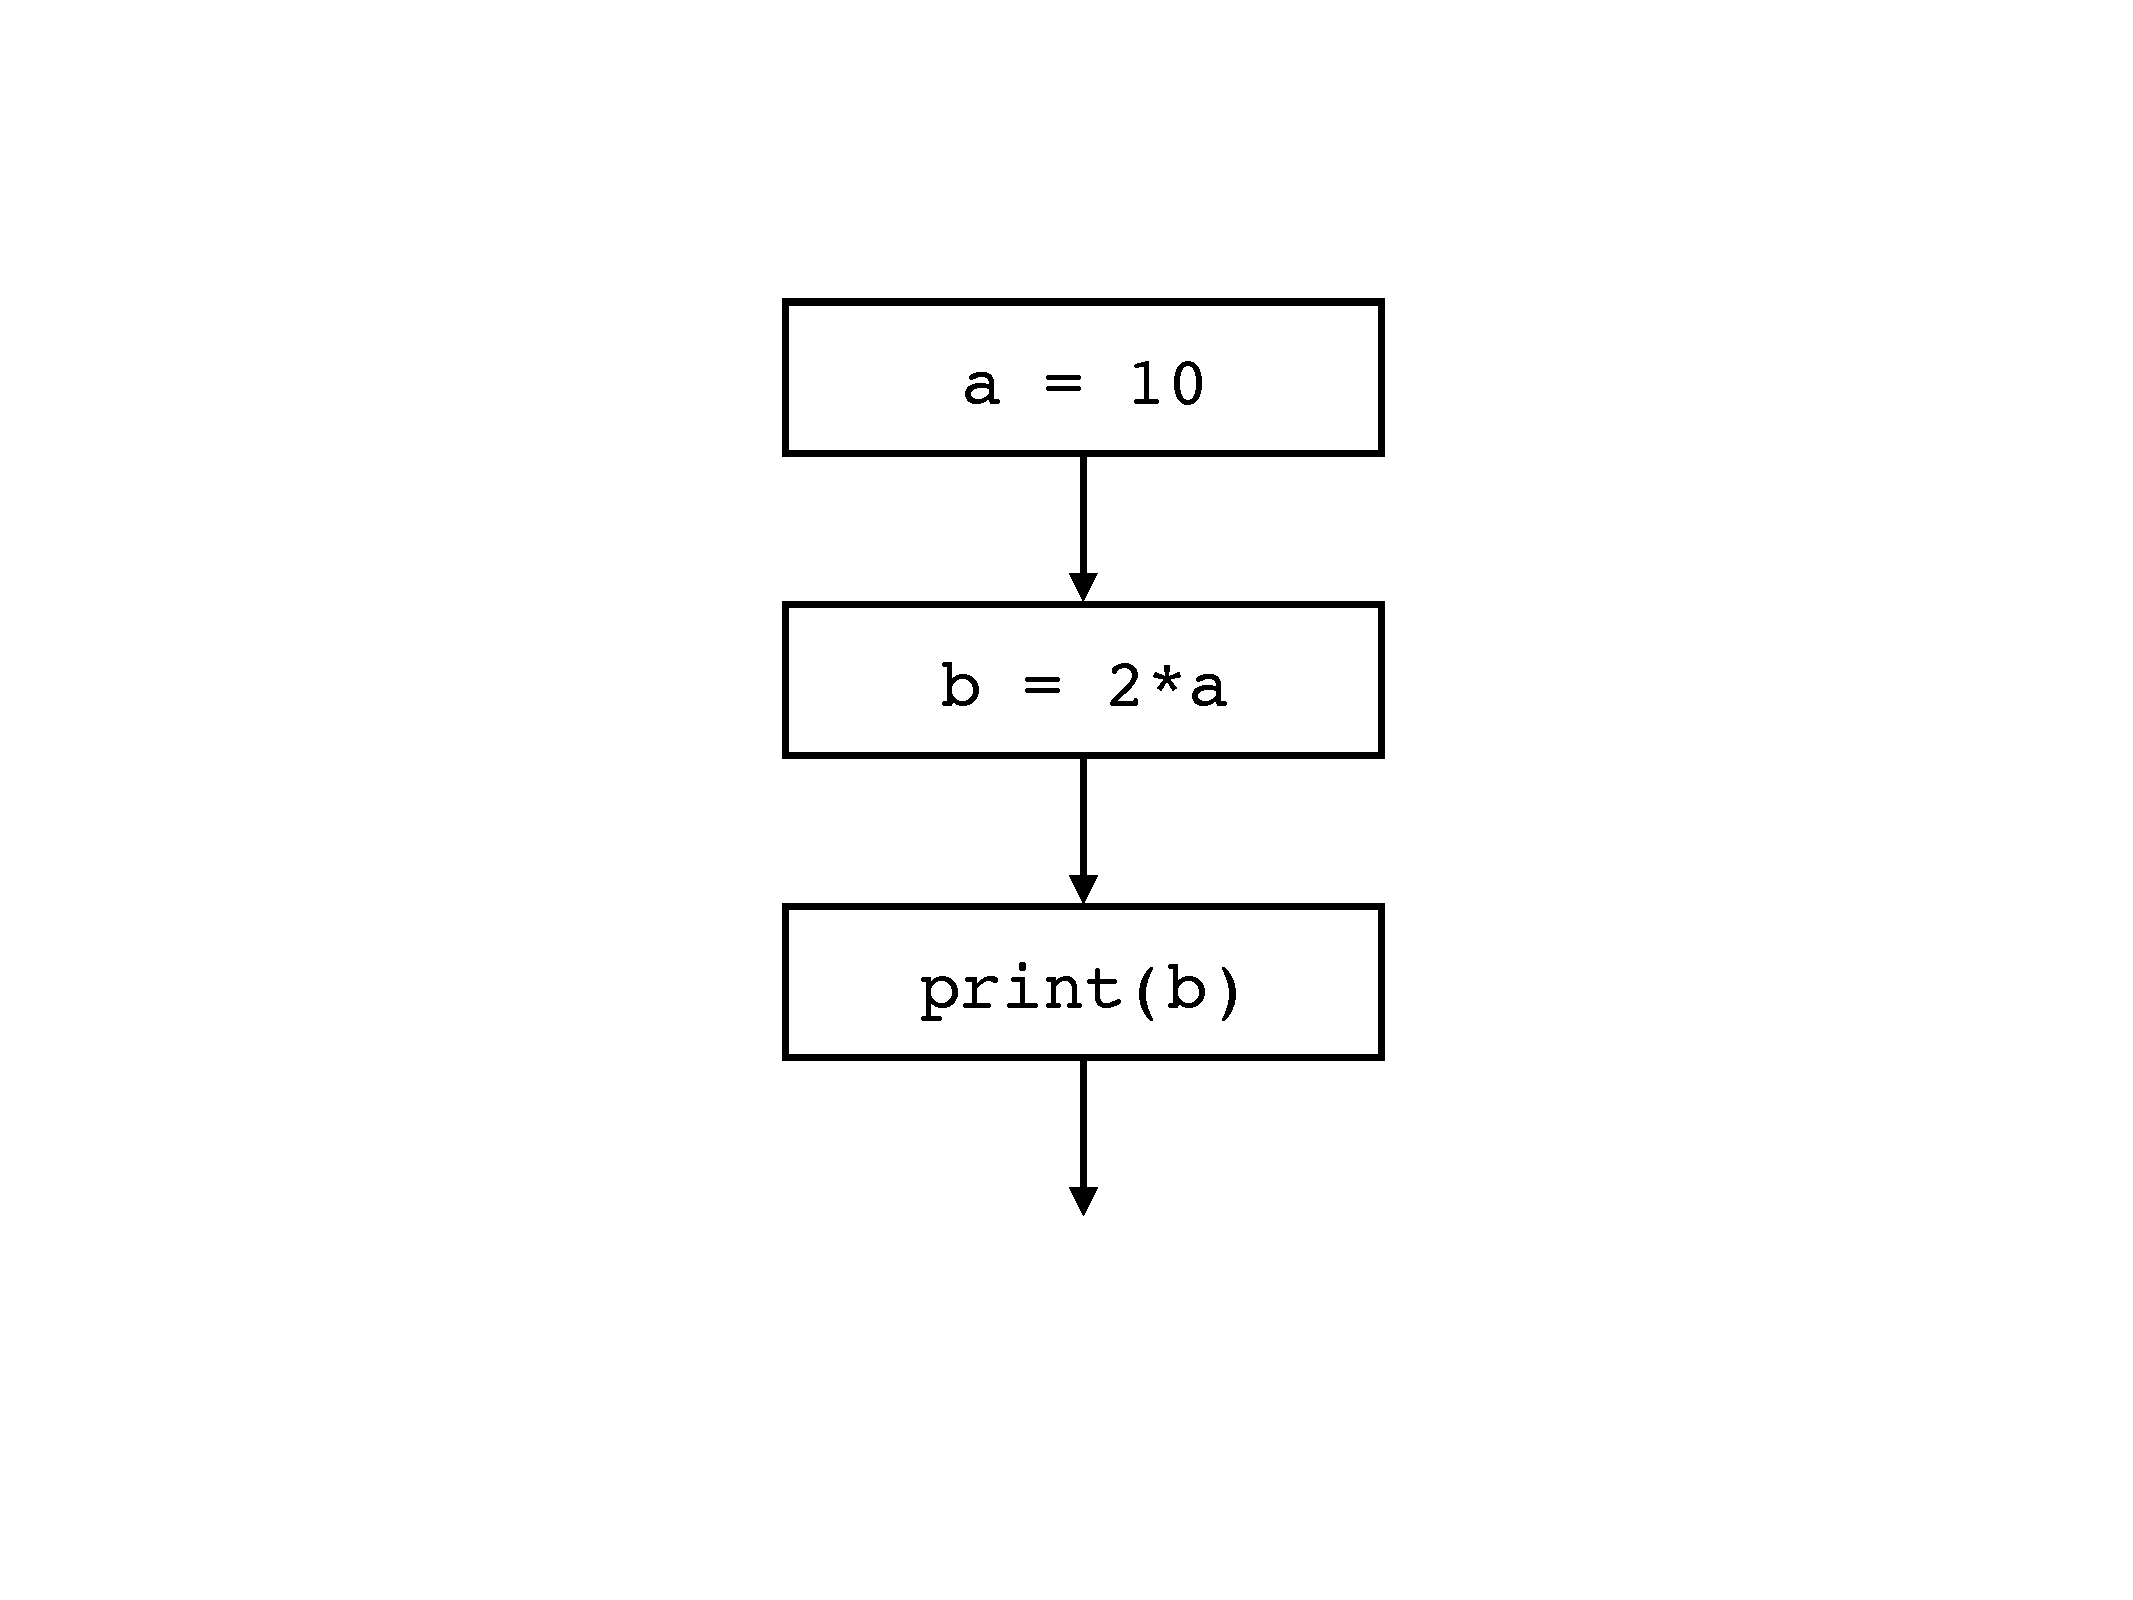
\includegraphics[height=2.5in]{{../Figures/sequential_program}.pdf}
\end{frame}

\begin{frame}[t]{If-Elif-Else}
	\begin{itemize}[<+->]
		\item Sequential programing is important, but cannot solve every problem.
	\end{itemize}
	\pause
    \centering
    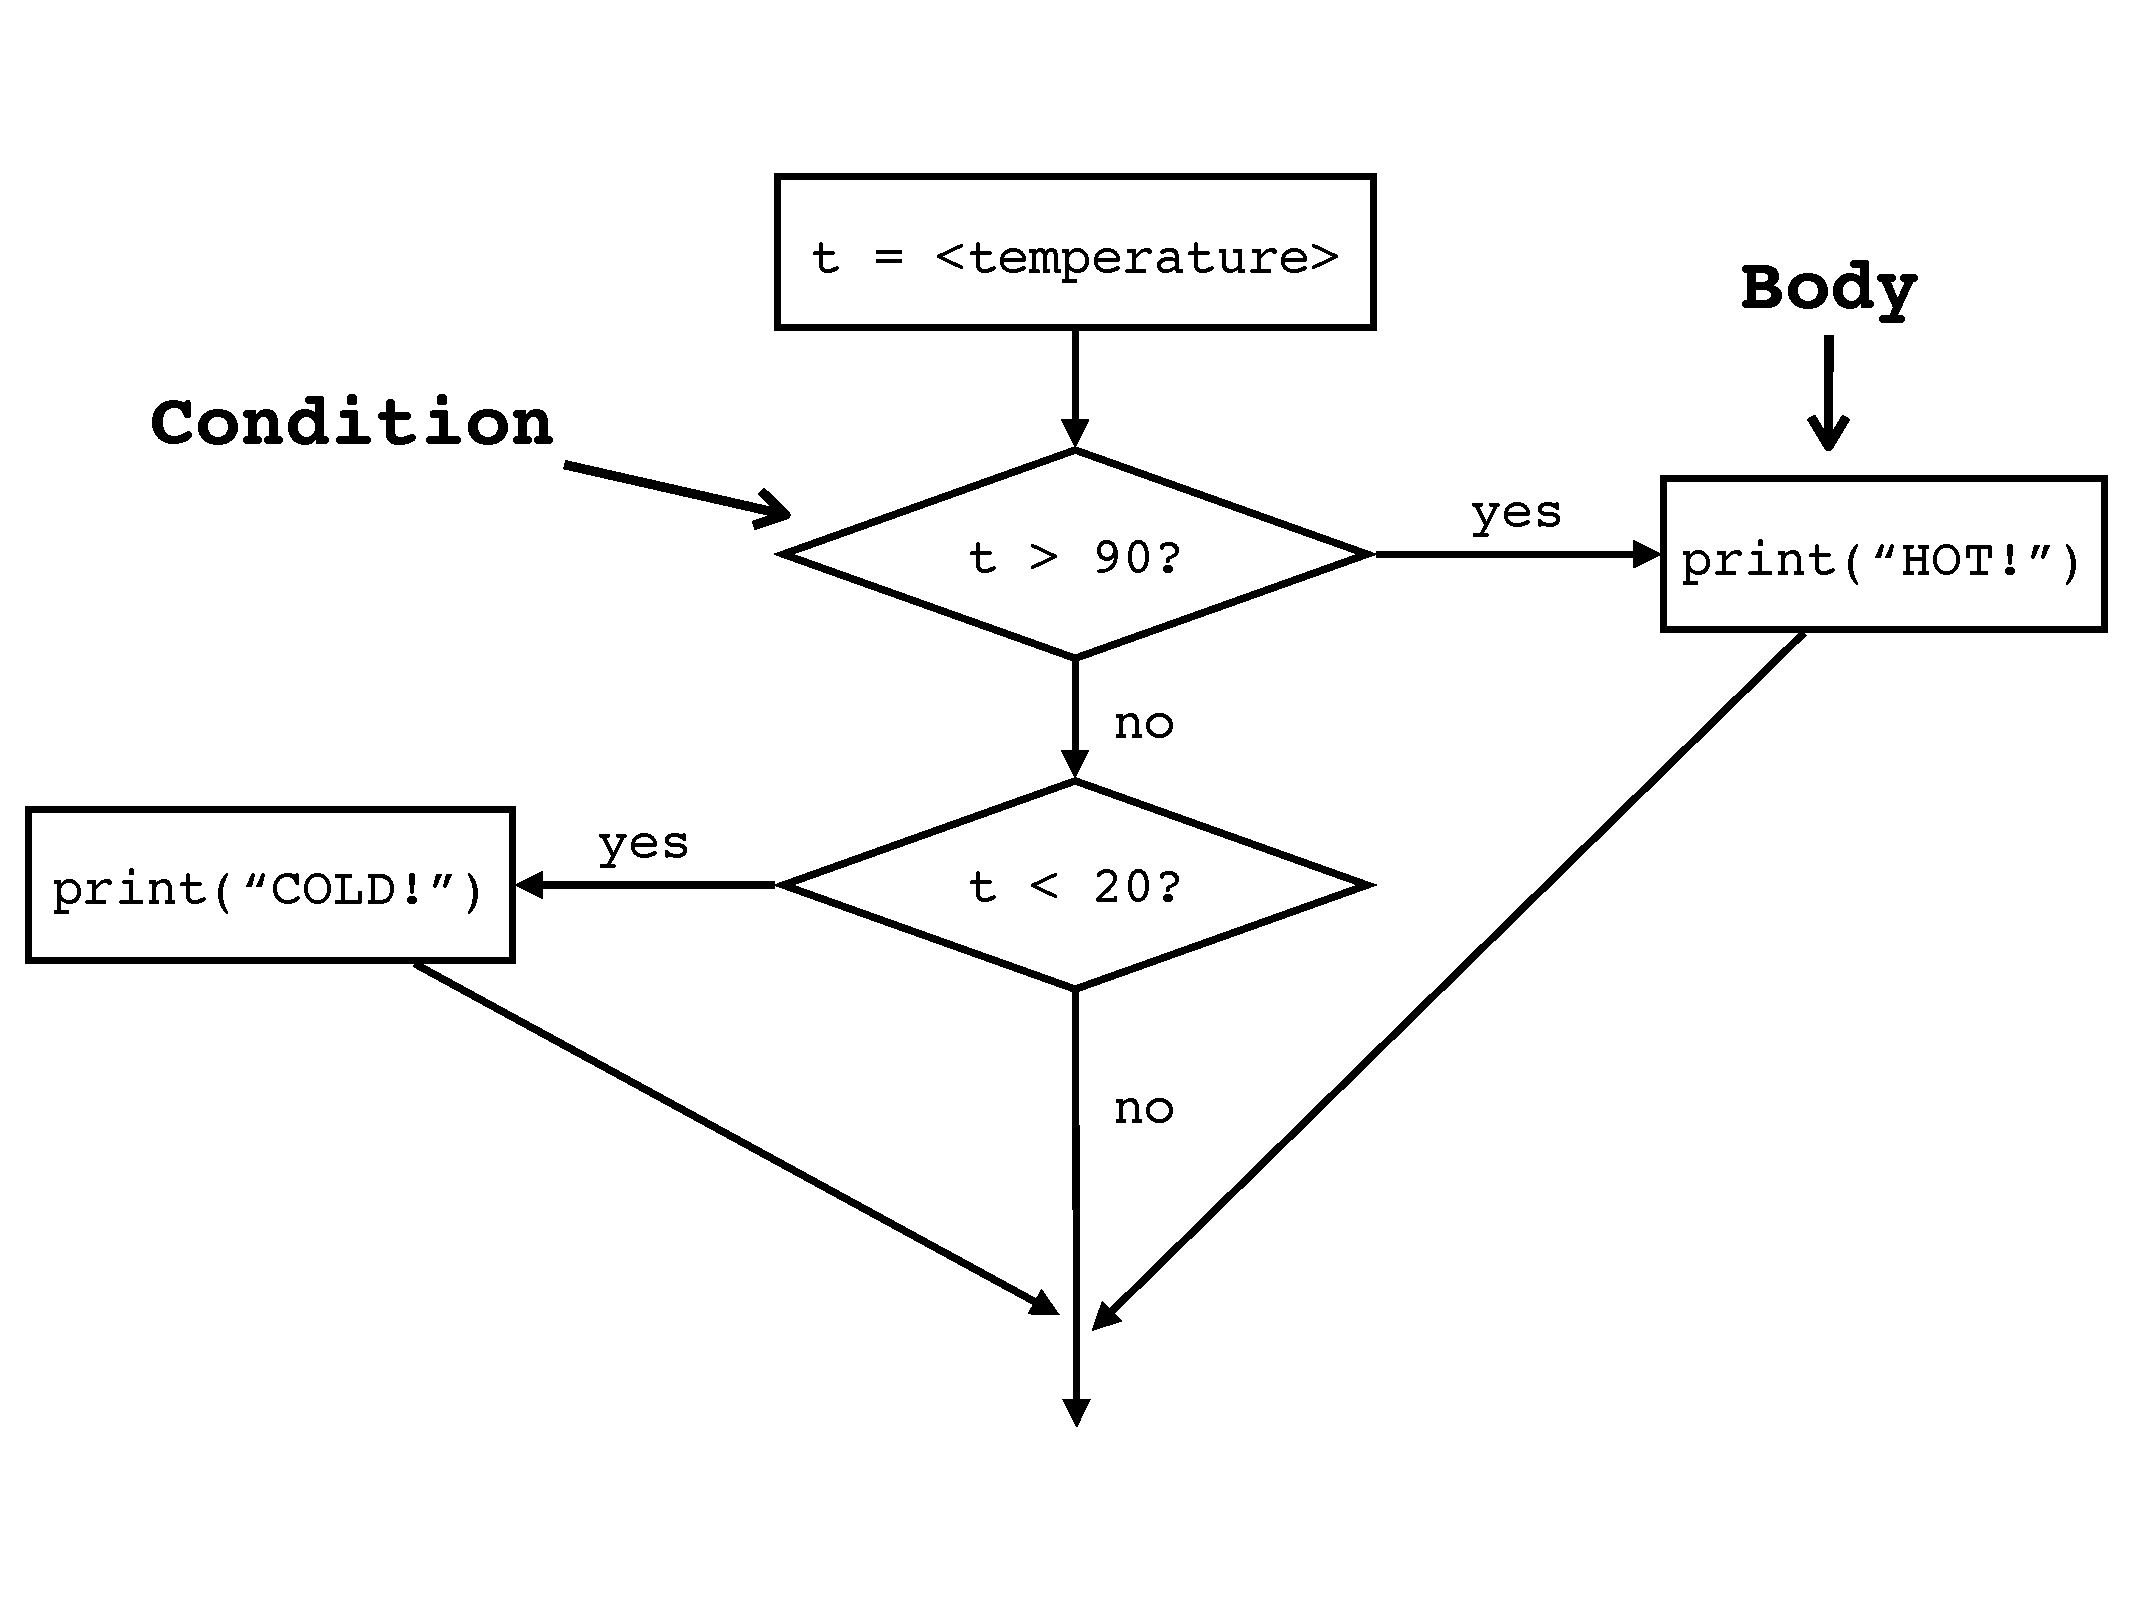
\includegraphics[height=2in]{{../Figures/conditional_program}.pdf}
\end{frame}

\begin{frame}[t,fragile]{If-Elif-Else}
	\begin{itemize}[<+->]
		\item If-Elif-Else statements allow us decide what code to execute depending on some conditions.
	\end{itemize}
	\pause
	\begin{tcolorbox}
		\begin{verbatim}
			if <condition1>:
			    <body1>
			elif <condition2>:
			    <body2>
			else:
			    <body3>
		\end{verbatim}
	\end{tcolorbox}
	\pause
	\centering
	\Huge{DEMO}
\end{frame}

\begin{frame}[t]{Loops}
	\begin{itemize}[<+->]
		\item Looping allow us run the same lines of code multiple times.
	\end{itemize}
	\pause
    \centering
    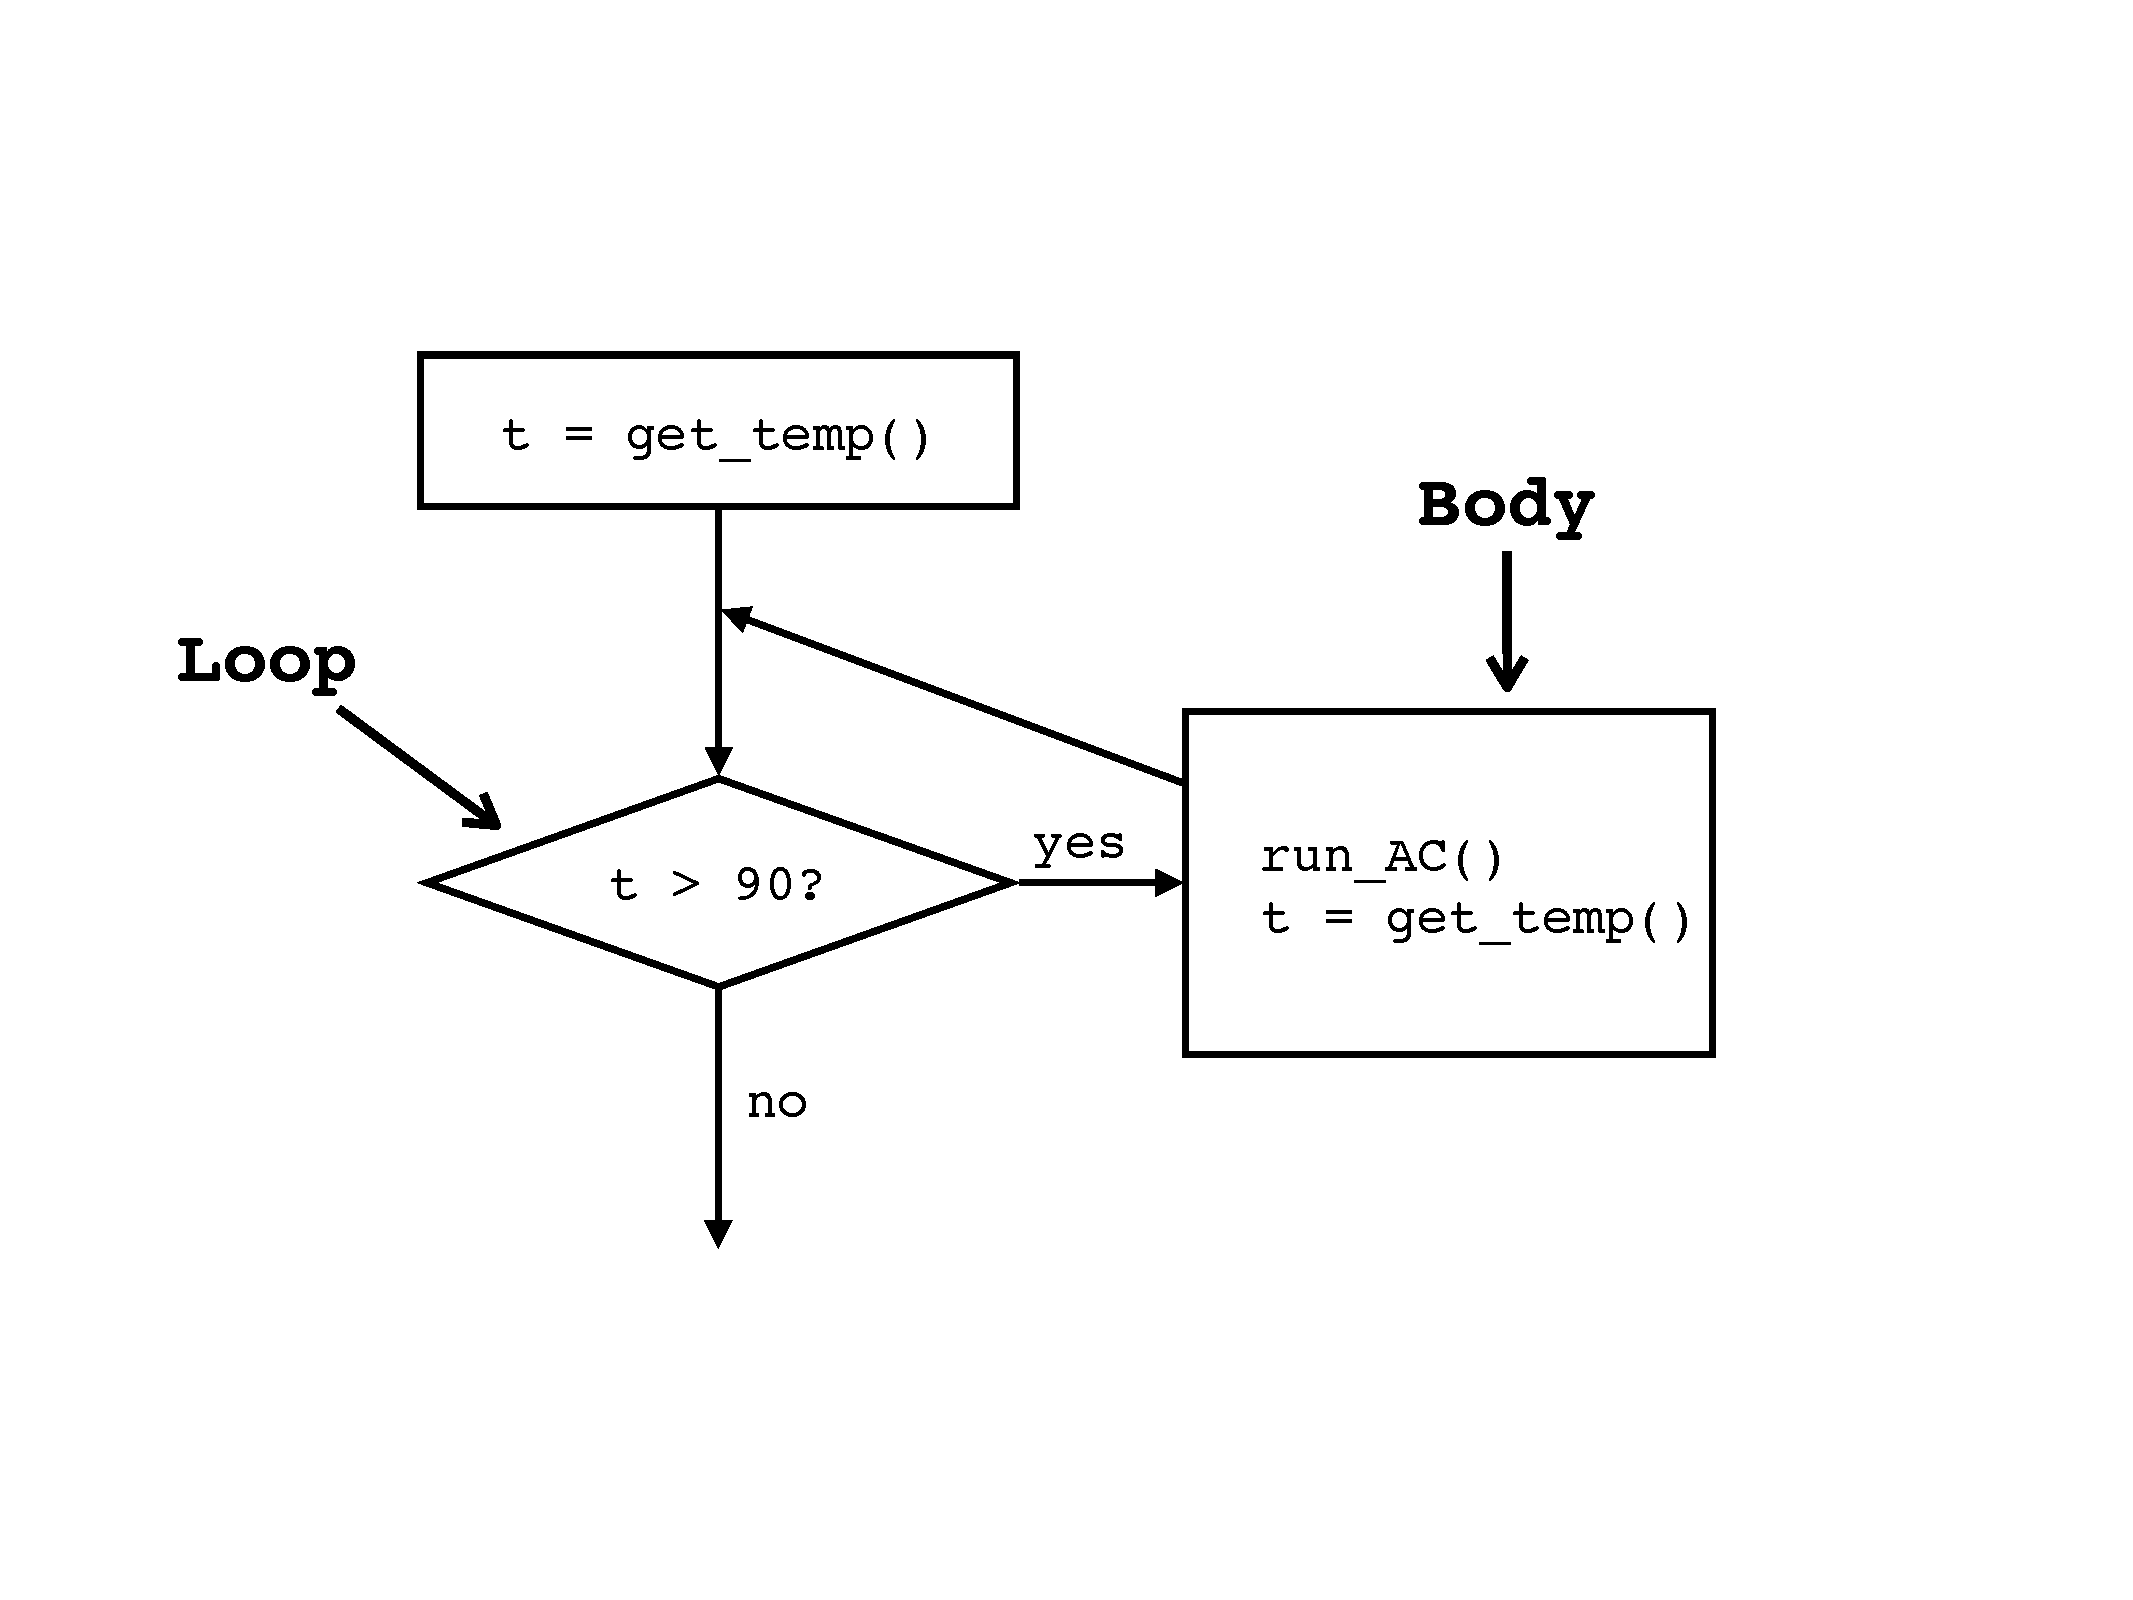
\includegraphics[height=2in]{{../Figures/loop_program}.pdf}
\end{frame}

\begin{frame}[t,fragile]{Loops}
	\begin{itemize}[<+->]
		\item There are two main types of loops in Python:
		\begin{itemize}[<+->]
			\item \textbf{For:} A block of code for every element in a sequence (list, tuple, or string).
		\end{itemize}
	\end{itemize}
	\pause
	\begin{tcolorbox}
		\begin{verbatim}
			for <var> in <sequence>:
			    <body>
		\end{verbatim}
	\end{tcolorbox}
	\pause
	\centering
	\Huge{DEMO}
\end{frame}

\begin{frame}[t,fragile]{Loops}
	\begin{itemize}
		\item There are two main types of loops in Python:
		\begin{itemize}
			\item \textbf{For:} A block of code for every element in a sequence (list, tuple, or string).
			\item \textbf{While:} A block of code as long as a condition is True.
		\end{itemize}
	\end{itemize}
	\pause
	\begin{tcolorbox}
		\begin{verbatim}
			while <condition>:
			    <body>
		\end{verbatim}
	\end{tcolorbox}
	\pause
	\centering
	\Huge{DEMO}
\end{frame}

% \begin{frame}[t]{Other types of conditionals}
%
%   \center
%   \Huge{Body}
% \end{frame}
\section{Functions}
\subsection{Foo}

\begin{frame}[t]{What is a function?}
	\begin{itemize}[<+->]
		\item Functions allow you to reuse portions of code.
		\item Functions can be thought of a sub-programs.
		\item Functions are \textit{called} or \textit{invoked}.
		\item Functions take \textit{parameters} and \textit{return a result}.
		\item We've already seen a number of built-in functions:
		\begin{itemize}[<+->]
			\item input
			\item print
			\item len
			\item open
			\item etc...
		\end{itemize}
	\end{itemize}
\end{frame}

\begin{frame}[t,fragile]{Defining Functions}
	\begin{itemize}[<+->]
		\item Functions are defined with the \textbf{def} statement.
	\end{itemize}
	\pause
	\begin{tcolorbox}
		\begin{verbatim}
			def <function_name>(<param1>,<param2>,...):
			    <body>
			    return <result>
		\end{verbatim}
	\end{tcolorbox}
	\pause
	\centering
	\Huge{DEMO}
\end{frame}

% \begin{frame}[t,fragile]{Example}
% 	\begin{itemize}[<+->]
% 		\item Functions are defined with the \textbf{def} statement.
% 	\end{itemize}
% 	\pause
% 	\begin{tcolorbox}
% 		\begin{verbatim}
% 			def <function_name>(<param1>, <param2>, ...):
% 				<body>
% 				return <result>
% 		\end{verbatim}
% 	\end{tcolorbox}
% 	\pause
% 	\centering
% 	\Huge{DEMO}
% \end{frame}

\begin{frame}[t]{Why use functions?}
	\begin{itemize}[<+->]
		\item Reuse code so you don't have to write it again.
		\item Provide an interface so others can use your code.
		\item Make code more compact and readable.
		\item \textbf{Only make changes once.}
	\end{itemize}
\end{frame}

\begin{frame}[t]{Functions and Parameters}
    \centering
    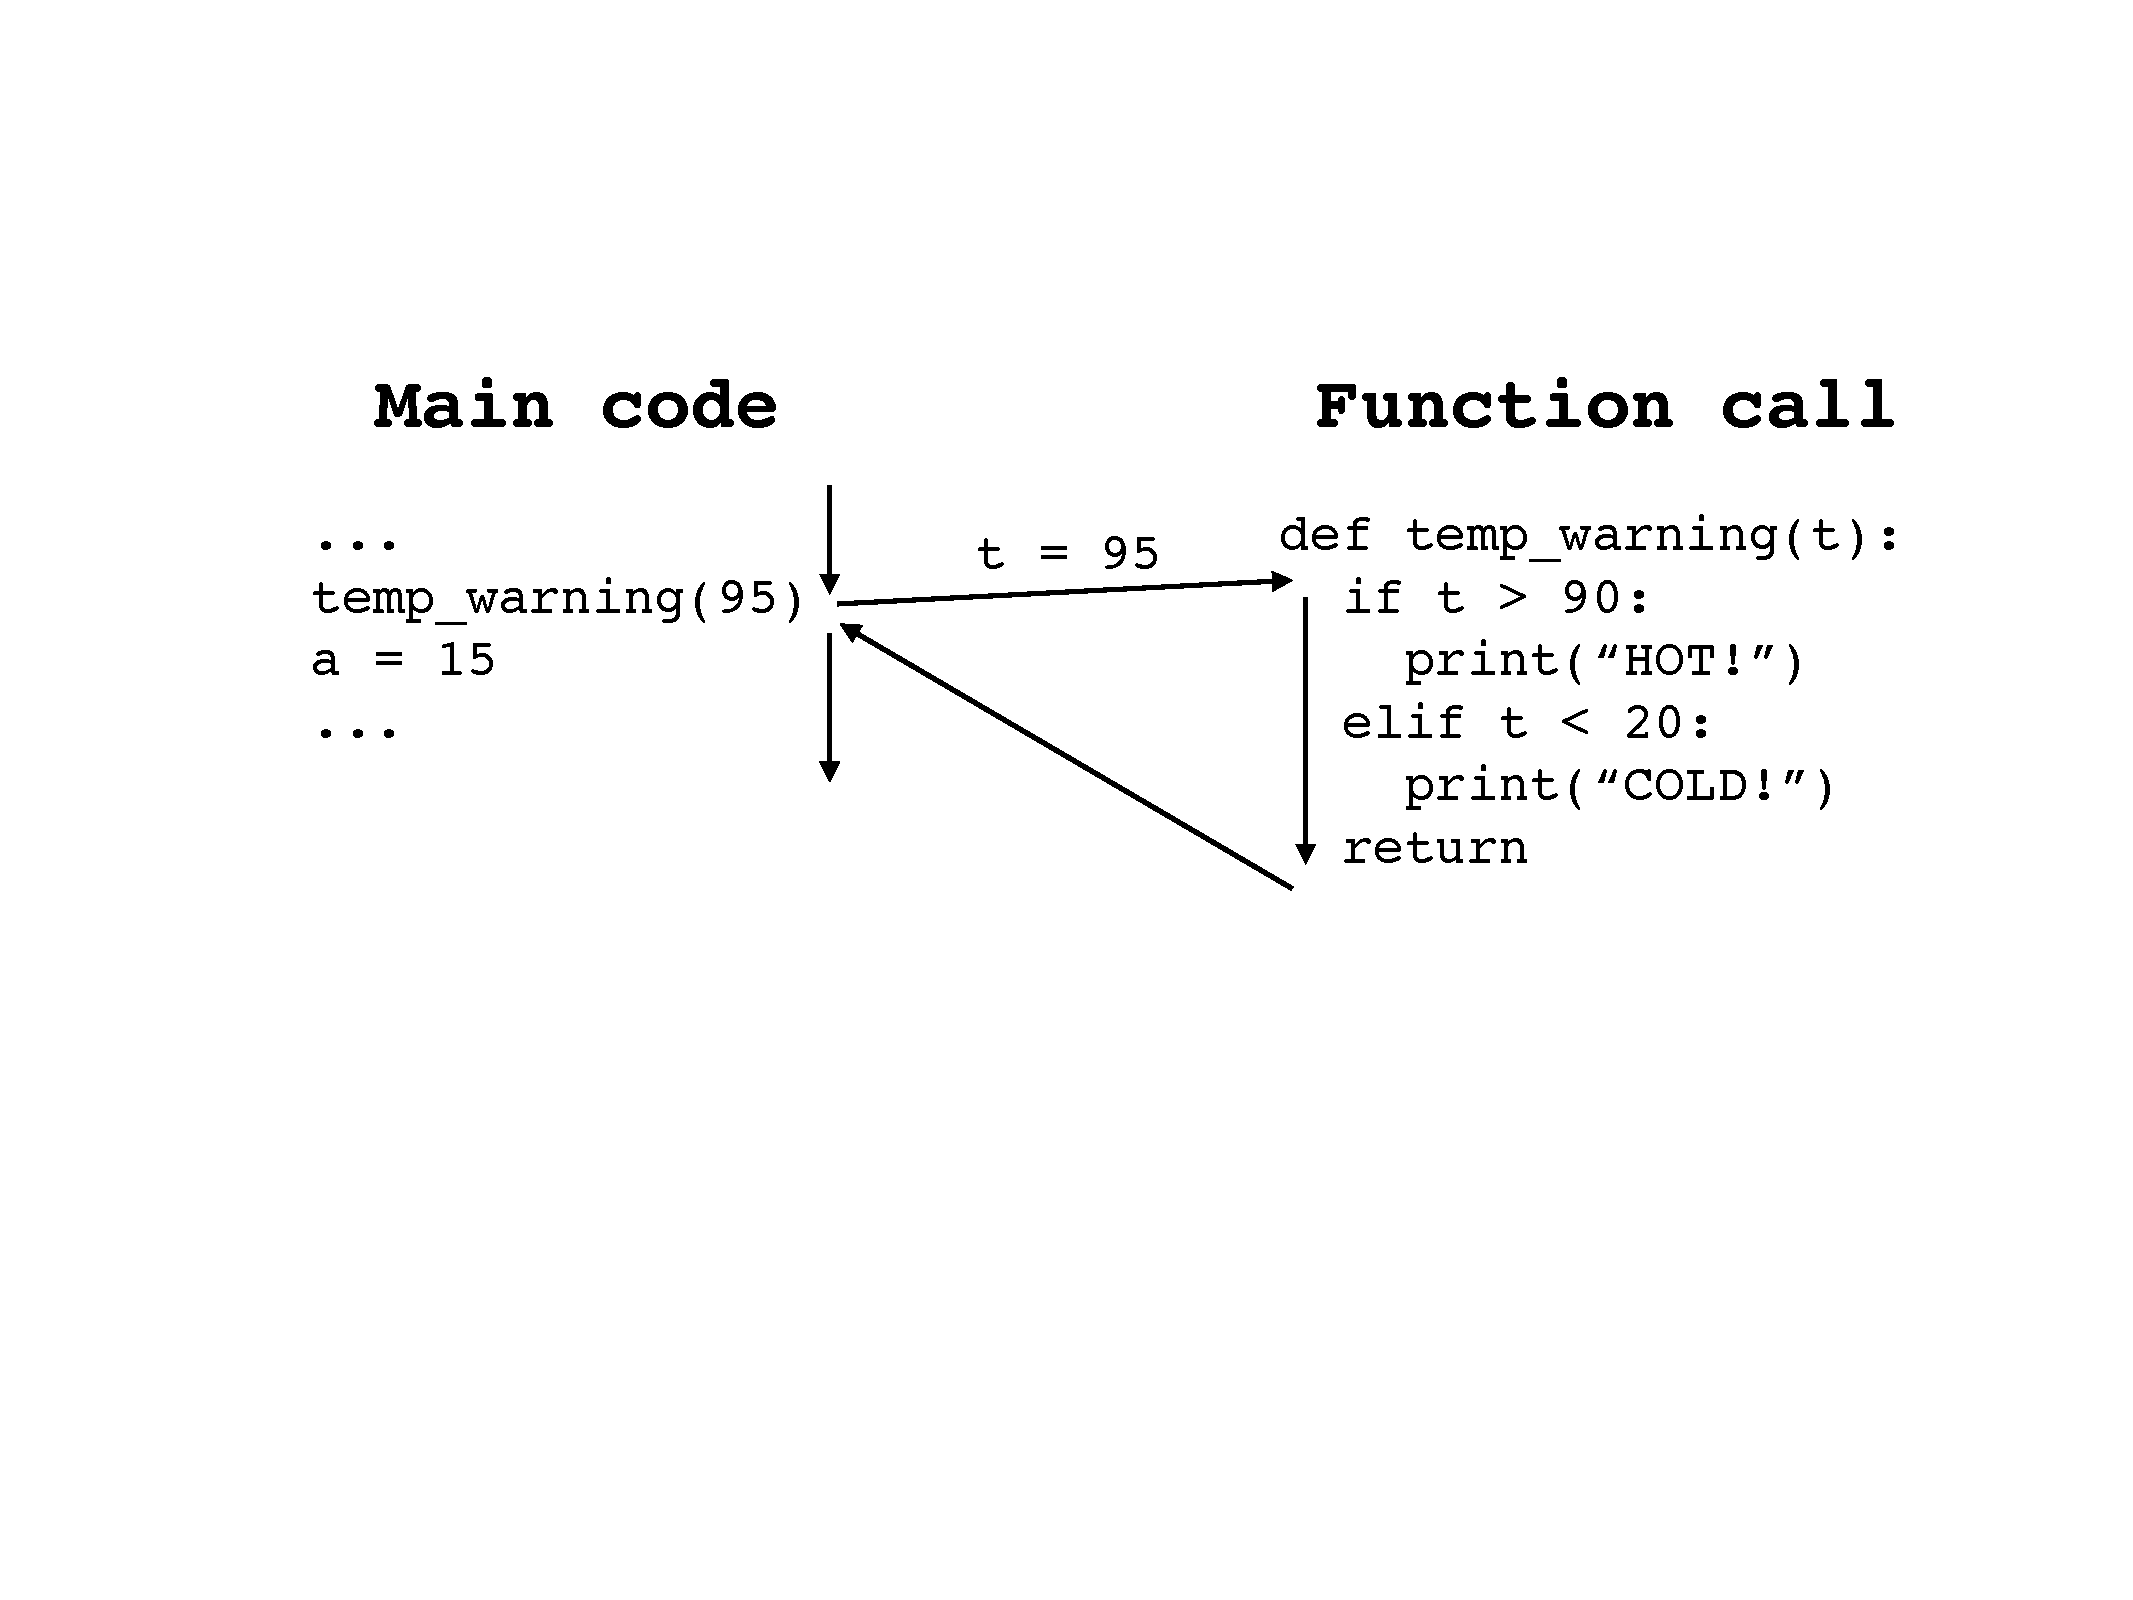
\includegraphics[width=4in]{{../Figures/function_call}.pdf}
\end{frame}

\section{Input and Output}
\subsection{Foo}

\begin{frame}[t]{Interaction}
	\begin{itemize}[<+->]
		\item Most programs must interact either with humans or other programs.
		\item Examples:
		\begin{itemize}[<+->]
			\item Interacting with the console or the mouse.
			\item Reading and writing files.
			\item Internet communications (we won't cover this).
		\end{itemize}
	\end{itemize}
\end{frame}

\begin{frame}[t,fragile]{Console I/O}
	\begin{itemize}[<+->]
		\item The easiest way to interact with the user is through the console.
		\item \textbf{input}: read text from the console.
		\item \textbf{print}: write text to the console.
	\end{itemize}

	\pause
	\begin{tcolorbox}
		\begin{verbatim}
			# Prompts user and reads until <return>
			user_input = input(<prompt>) 
			
			# print arguments separated by spaces
			print(<print_string1>,<print_string2>,...) 
		\end{verbatim}
	\end{tcolorbox}
	\pause
  \centering
  \Huge{DEMO}
\end{frame}

\begin{frame}[t,fragile]{File I/O}
	\begin{itemize}[<+->]
		\item We can save results and interact with other programs through the file system.
		\item \textbf{open}: open a file.
		\item \textbf{read}: read the contents of a file.
		\item \textbf{write}: write to a file.
		\item \textbf{close}: close a file.
	\end{itemize}
	\pause
	\begin{tcolorbox}
		\begin{verbatim}
			file = open(<file_name>, <mode>) 
			file_contents = file.read()
			file.write(<output>) 
			file.close() 
		\end{verbatim}
	\end{tcolorbox}
	\pause
  \centering
  \Huge{DEMO}
\end{frame}



% \begin{frame}[t]{Scoping in Python}
% 	Variables defined wi
%   \center
%   \Huge{Body}
% \end{frame}

\begin{frame}[t,fragile]{Importing Functions}
	\begin{itemize}[<+->]
		\item \textbf{Modules} are Python code, usually and collection of functions, that can be used in other programs.
		\item Load modules into your code using an \textbf{import} statement.
	\end{itemize}
	\pause
	\begin{tcolorbox}
		\begin{verbatim}
			import <module_name> # imports a module
		\end{verbatim}
	\end{tcolorbox}
	\pause
	\centering
	\Huge{DEMO}
\end{frame}

% \section{Classes and Objects}
% \subsection{Foo}

\end{document}
